%! TEX root = main.tex

%/========== Variable Length Pendulum ==========/%
\chapter{Application of VNHCS: The Variable Length Pendulum}\label{sec:vlp}
\section{Motivation}
The variable length pendulum (VLP) is a classical underactuated dynamical system
which is often used to model the motion of a person on a swing
\cite{pumping_swing_standing_squatting,how_to_pump_a_swing}.
The VLP also represents the motion of the load at the end of a crane, 
the (simplified) motion of a gymnast on a bar
\cite{pendulum_length_giant_gymnastics}, and the tuned-mass-damper systems which
stabilize skyscrapers \cite{vlp_tuned_mass_damper}.

The motion of the VLP has been well studied (see for instance
\cite{dynamics_periodic_vlp}), and many control mechanisms exist
to stabilize trajectories of the system. While many of these controllers 
are time-dependent, \citet{vlp_energy_shaping}
offer a time-independent technique to inject energy into the VLP. 
They designed a controller through a technique called \textit{energy shaping},
and proved that their control mechanism stabilizes any desired energy level set.
However, the energy injection mechanism is ad-hoc in the sense that it is not
derived from natural behaviour. 
In this chapter we will design VNHCs to stabilize energy levels of the VLP in a
time-independent manner, while maintaining the structured motion of a human on a
swing.

\section{Dynamics of the Variable Length Pendulum}
% Derive the dynamics of the VLP in Hamiltonian form
We will model the VLP as a point mass \(m\)
connected to a fixed pivot by a massless rod of varying length \(l\) with angle 
\(q \in \mathbb{S}^1\) from the vertical, as is seen in Figure
\ref{fig:vlp-model}. 
We will also ignore any damping and frictional forces in this model.
In a realistic VLP, the rod length \(l\) varies between some minimum
length \(\underline{l} \geq 0\) and some maximum length 
\(\overline{l} > \underline{l}\). The configuration of the VLP is the vector
\(\mathbf{q} := (q,l) \in \mathbb{S}^1 \times [\underline{l},\overline{l}]\).

\begin{figure}
   \centering
   \includestandalone[width=0.5\textwidth]{images/vlp_model}
   \caption{The variable length pendulum is a mass attached to the
      tip of a massless rod which can change length.}\label{fig:vlp-model}
\end{figure}

Using this configuration, we will compute the Hamiltonian dynamics of the system.
The cartesian position of the mass at the tip of the pendulum
is given by \(x = (l\sin(q),-l\cos(q))\), while its velocity is
\(\dot{x} = (\dot{l}\sin(q) + l\cos(q)\dot{q}, -\dot{l}\cos(q) + l\sin(q)\dot{q})\).
Computing the kinetic energy \(T\) yields
\[
   T(\mathbf{q},\dot{\mathbf{q}}) = 
   \frac{1}{2}m\norm{\dot{x}}^2 = \frac{1}{2}m\left(\dot{l}^2 + l^2\dot{q}^2\right)
\]
The potential energy \(P\) with respect to the pivot (under a gravitational
acceleration \(g\)) is
\[
   P(\mathbf{q}) = -mgl\cos(q)
\]
Collecting the kinetic energy into a quadratic form, we get the Lagrangian
\[
   \mathcal{L}(\mathbf{q},\dot{\mathbf{q}}) 
   = \frac{1}{2} \dot{\mathbf{q}}\tpose D(\mathbf{q})\dot{\mathbf{q}} - P(\mathbf{q})
   = \frac{1}{2}
   \begin{bmatrix} \dot{q} & \dot{l} \end{bmatrix}
   \begin{bmatrix}
      ml^2 & 0 \\
      0 & m \\
   \end{bmatrix}
   \begin{bmatrix} 
      \dot{q} \\ \dot{l}
   \end{bmatrix}
   + mgl\cos(q)
\]
Computing the conjugate of momenta to \(\mathbf{q}\), we get 
\[
   \mathbf{p} := \begin{bmatrix} p \\ p_l \end{bmatrix} 
   = \begin{bmatrix} ml^2\dot{q} \\ m\dot{l} \end{bmatrix} 
\]
Performing the Legendre transform on \(\mathcal{L}\) and setting
\(M(\mathbf{q}) := D(\mathbf{q})\), \(V(\mathbf{q}) := P(\mathbf{q})\),
we find the Hamiltonian is equal to the total mechanical energy of the system:
\[
   \mathcal{H} = E = \frac{1}{2}\mathbf{p}\tpose \Minv(\mathbf{q})
   \mathbf{p}+V(\mathbf{q})
\]
Taking the appropriate derivatives, the dynamics of the VLP in Hamiltonian form
are described in (\ref{eqn:vlp-hamiltonian-with-pl}). 
\begin{align}\label{eqn:vlp-hamiltonian-with-pl}
   \mathcal{H} &= \frac{1}{2} \begin{bmatrix} p & p_l \end{bmatrix}
      \begin{bmatrix}
         \frac{1}{ml^2}  & 0 \\
         0 & \frac{1}{m}
      \end{bmatrix} \begin{bmatrix} p \\ p_l \end{bmatrix} - mgl\cos(q) \\
     &\begin{cases}
        \dot{q} = \frac{p}{ml^2} \\
        \dot{l} = \frac{p_l}{m} \\
        \dot{p} = -mgl\sin(q) \\
        \dot{p}_l = \frac{p^2}{ml^3} + mg\cos(q) + \tau \\
   \end{cases} \nonumber
\end{align}
The control input is a force \(\tau \in \mathbb{R}\) affecting the dynamics of
\(p_l\), acting colinearly with direction of the rod.
We assume the force does not affect the dynamics of \(p\) in any way -
that is, the control input cannot enact any lateral force on the pendulum.
This is extremely useful for simplifying the dynamics: since one can choose
\(\tau\) which sets \(\dot{p}_l\) to any desired function and \(\dot{l}\)
depends only on \(p_l\), we can assume (with abuse of notation) that \(l\) is
tracking some known function \(l(t)\). 
The closed loop dynamics of the system will be described exclusively by
\((\dot{q},\dot{p})\) with \(l \equiv l(t)\).
The fact that \(p_l\) does not appear in these closed-loop dynamics allows us to
ignore the subdynamics \((\dot{l},\dot{p}_l)\) entirely. 

What this means is we can treat \(l\) as the control input directly, rather than
modelling it as a configuration variable. Re-deriving the Hamiltonian and the
dynamics from this approach, we get the system 
(\ref{eqn:vlp-hamiltonian}) with phase \((q,p) \in \mathbb{S}^1 \times \R\). 
Note that the control input \(l(t)\) and its derivative \(\dot{l}(t)\) are both
known variables.
\begin{align}\label{eqn:vlp-hamiltonian}
   \mathcal{H}(q,p) &= \frac{p^2}{ml^2} - \frac{1}{2}\dot{l}^2 - mgl\cos(q) \\
     &\begin{cases}
        \dot{q} = \frac{p}{ml^2} \\
        \dot{p} = -mgl\sin(q) \\
      \end{cases}\nonumber
\end{align}
In particular, the Hamiltonian of this simplified model is no longer equal to
the total mechanical energy of the system, which is given by
(\ref{eqn:vlp-energy}).
\begin{equation}\label{eqn:vlp-energy}
   E(q,p) = \frac{p^2}{ml^2} + \frac{1}{2}\dot{l}^2 - mgl\cos(q)
\end{equation}

% TODO: Describe the oscillation and rotation motion of a pendulum in the
% qp-plane, and give a figure showing the orbiting motion for each of these.
% Then describe what the orbit should do under energy injection (spiral away /
% begin rotation outward) and energy dissipation (spiral in / rotate inward).

\section{The VLP Constraint}
% Go through the development of the constraint and prove it gains energy
To motivate why a VNHC could inject energy into the VLP in a human-like
manner, we will examine a person standing on a swing.
As can be seen in Figure \ref{fig:child-vlp}, their center of mass moves closer
to the swing's pivot when they stand, and moves away from the pivot when they
squat.
This is equivalent to the VLP model from Figure \ref{fig:vlp-model}, where
standing and squatting correspond to shortening and lengthening the pendulum
(respectively).
\begin{figure}
   \centering
   \begin{subfigure}[t]{0.45\textwidth}
      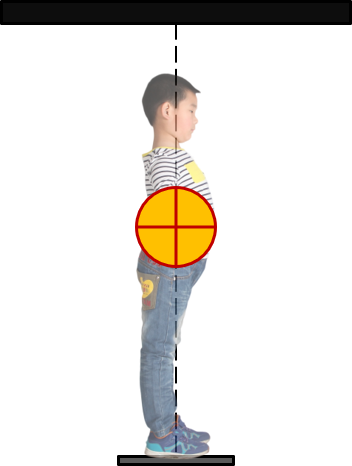
\includegraphics[]{images/child_vlp_standing.png}
      \caption{A person standing on a swing has their center of mass 
      close to the pivot.}
   \end{subfigure}
   \hfill
   \begin{subfigure}[t]{0.45\textwidth}
      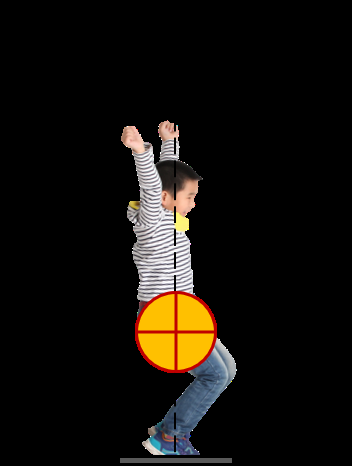
\includegraphics[]{images/child_vlp_squatting.png}
      \caption{When a person squats on a swing, their center of mass extends
      away from the pivot.}
   \end{subfigure}
   \caption{The VLP representation of a person on a standing swing.}
   \label{fig:child-vlp}
\end{figure}

The action of regulating pendulum length to add energy to the VLP is known as
``pumping". \citet{pumping_swing_standing_squatting} asked whether
the pumping strategy performed by children is time-optimal, assuming the
children could squat or stand instantaneously. 
Indeed, they discovered that children increase the height of their swing as fast
as is physically possible.

A child's optimal pumping strategy is the following: 
they stand at the lowest point of the swing, and squat at the highest point.
Looking at the VLP representation, the pendulum shortens at the bottom of the
swing, and lengthens at the top. 
For an intuitive explanation, conservation of angular momentum indicates that
shortening the pendulum at the bottom forces the mass to gain speed to
compensate for the reduced length \cite{how_to_pump_a_swing}.
Energy is not conserved in this process, so the pendulum gains kinetic energy
and reaches a higher point at the peak of its swing.
Lengthening the pendulum when it reaches this peak means gravity
imparts a larger angular momentum to the mass by the time it reaches the bottom
of its swing, which in turn is converted to a higher velocity when the
pendulum is shortened.
By alternating these processes, the pendulum experiences an average net gain in
rotational energy.

Notice that the child's pumping strategy requires knowledge of
when the system is at the ``bottom" or ``top" of the swing. 
Since being at the ``bottom" is equivalent to having angle \(q = 0\) and being
at the ``top" is equivalent to having momentum \(p = 0\), a controller based on
this strategy will necessarily use the full phase \((q,p)\). 
This is why we will use VNHCs instead of VHCs.

The time-optimal controller from \cite{pumping_swing_standing_squatting} is (in
our notation)
\[
   l_\text{opt}(q,p) := -\sign{qp}
\]
which is a piecewise-continuous controller that varies between \(\pm 1\). 
This looks similar to a VNHC, but it is not smooth and makes the assumption that 
\(l \in [-1,1]\). 
Since we want our controller emulate realistic human motion, we need to derive a
smooth controller where we allow \(l \in [\underbar{l},\overbar{l}]\); then, we
will prove that it injects energy.

Figure \ref{fig:vlp-optimal-controller-qp-plane} displays \(l_\text{opt}\) 
directly on the \((q,p)\)-plane.
Because the length remains constant inside each quadrant and changes only when it
crosses one of the axes, one can use the angle \(\theta = \arctan_2(p,q)\) to
redefine the time-optimal controller in a way which is easier to ``smooth out".
Figure \ref{fig:vlp-optimal-controller} shows the time-optimal pumping strategy
as a function \(l^\star(\theta)\) (\ref{eqn:vlp-optimal-controller}), where now
the length varies between \([\underbar{l},\overbar{l}]\) rather than 
\([-1,1]\). 

\begin{equation}\label{eqn:vlp-optimal-controller}
   l^\star(\theta):= \begin{cases}
      \overline{l} & \theta \in [-\frac{\pi}{2},0[ \cup [\frac{\pi}{2}, \pi[ \\
      \underline{l} & \theta \in [-pi, -\frac{\pi}{2}[ \cup [0,\frac{\pi}{2}[ \\
   \end{cases}
\end{equation}

\begin{figure}
   \centering
   \begin{subfigure}[t]{0.45\textwidth}
      \includestandalone[width=\linewidth]{images/vlp_optimal_controller_qp_plane}
      \caption{The time-optimal controller \(l_\text{opt}\) mapped onto the \((q,p)\)-plane.}
      \label{fig:vlp-optimal-controller-qp-plane}
   \end{subfigure}
   \hfill
   \begin{subfigure}[t]{0.45\textwidth}
      \includestandalone[width=\linewidth]{images/vlp_optimal_controller}
      \caption{The time-optimal controller converted to the alternate
         representation \(l^\star(\theta)\).}
      \label{fig:vlp-optimal-controller}
   \end{subfigure}
   \caption{The time-optimal controller for a standing swing as derived by
      \cite{pumping_swing_standing_squatting}. The colour red
      corresponds to standing, blue to squatting, and 
      \(\theta := \arctan_2(p,q)\) is the angle of the VLP phase in the
      \((q,p)\)-plane.}
\end{figure}

We now define a continuous function which
approximates \(l^\star(\theta)\) by attaching sinusoids at the
discontinuities (see Figure \ref{fig:vlp-T-controller}). 
Let \(\Delta l := (\overline{l} - \underline{l})/2\) and 
\(l_{\text{avg}} := (\overline{l} + \underline{l})/2\).
Providing these newly attached sinusoids with a frequency \(\omega = \frac{\pi}{T}\) 
(where \(T \in \, ]0,\frac{\pi}{2}]\) is a control parameter), we get the
continuously-differentiable controller \(l_T(\theta)\) (\ref{eqn:vlp-T-controller}).
\begin{equation}\label{eqn:vlp-T-controller}
   l_T(\theta) = \begin{cases}
      \overline{l} & \theta \in \left[-\frac{\pi}{2} + \frac{T}{2}, -\frac{T}{2}\right] 
      \cup \left[\frac{\pi}{2} + \frac{T}{2}, \pi - \frac{T}{2}\right] \\
      \underline{l} & \theta \in \left[-\pi + \frac{T}{2}, -\frac{\pi}{2} - \frac{T}{2}\right] 
      \cup \left[\frac{T}{2}, \frac{\pi}{2} - \frac{T}{2}\right] \\
      -\Delta l \sin(\omega(\theta + \pi)) + l_{\text{avg}} & \theta \in
      \left[-\pi,-\pi + \frac{T}{2}\right] \\
      -\Delta l \sin(\omega \theta) + l_\text{avg} & \theta \in [-\frac{T}{2},
      \frac{T}{2}] \\
      \Delta l \sin(\omega(\theta - a)) + l_\text{avg} & 
      \theta \in \left[a - \frac{T}{2}, a + \frac{T}{2}\right] \text{ for } 
      a \in \left\{-\frac{\pi}{2}, \frac{\pi}{2}\right\} \\
      -\Delta l \sin(\omega(\theta-\pi)) & \theta \in \left[\pi - \frac{T}{2},\pi\right] \\
   \end{cases}
\end{equation}

\begin{figure}
   \centering
   \includestandalone[width=0.7\textwidth]{images/vlp_T_controller}
   \caption{The continuous VNHC-style VLP controller \(l_T(\theta)\).}\label{fig:vlp-T-controller}
\end{figure}

This controller approximates the optimal controller because 
\[
   \lim\limits_{T \rightarrow 0} l_T(\theta) = l^\star(\theta)
\]
Unfortunately, while \(l_T(\theta)\) is continuously-differentiable, 
it is not twice-differentiable for most values of \(T\).
If we wish to use it as a VNHC, we must ensure that either the generalized
forces \(\tau\) acting on \(p_l\) can be discontinuous (which is certainly
achievable by humans), or we must find a value of \(T\) where this controller is
smooth.
Thankfully, \(l_{\frac{\pi}{2}}(\theta)\) is smooth as it can be simplified into
the expression (\ref{eqn:vlp-smoothed-controller}). 
\begin{equation}\label{eqn:vlp-smoothed-controller}
   l_\frac{\pi}{2}(\theta) = -\Delta l \sin(2\theta) + l_{\text{avg}}
\end{equation}
It is plotted for demonstration in Figure \ref{fig:vlp-smoothed-controller}.

\begin{figure}
   \centering
   \includestandalone[width=0.6\textwidth]{images/vlp_smoothed_controller}
   \caption{The smoothed VLP controller which corresponds to the VNHC \(l =
      l_\frac{\pi}{2}(\theta)\).}\label{fig:vlp-smoothed-controller}
\end{figure}

Because \(l_\frac{\pi}{2}(\theta)\) is smooth and it approximates
\(l^\star(\theta)\), we set our VNHC to be
\[
   h(q,p) = l - l_\frac{\pi}{2}\left(\theta(q,p)\right)
\]
We still need to prove this VNHC will inject energy into a VLP. 
Before we can do this, we require the following lemma.

\begin{lemma}\label{lemma:sign-of-cube}
   For any \(x,y \in \R\):
   \[
      \sign{x^3 - y^3} = \sign{x-y}
   \]
\end{lemma}
\begin{proof}
   Observe first that
   \[
      x^3 - y^3 =  (x-y)(x^2 + xy + y^2)
   \]
   The inequality \(x^2 + xy + y^2 \geq 0\) holds because
   \[
      x^2 + xy + y^2 = \left(x  + \frac{y}{2}\right)^2 + \frac{3y^2}{4} \geq 0
   \]
   which proves the lemma.
\end{proof}

Supposing the initial condition is not an equilibrium, we will show that the
constrained dynamics trace out a curve on the \((q,p)\)-plane which is diverging
from the origin.  
This implies that the momentum \(p\) is increasing in magnitude whenever the
curve hits the \(p\)-axis, which in turn means the VLP is gaining energy on
average.

\begin{thm}\label{thm:vlp-energy-stabilization}
   Take the VLP (\ref{eqn:vlp-hamiltonian}) with initial condition 
   \((q_0,p_0) \not \in \left\{(0,0),(\pm\pi,0)\right\}\).
   Define \(\theta := \arctan_2(p,q)\). 
   A VNHC of the form \(h(q,p) = l - l(\theta)\) injects energy if there exists 
   \(l_\text{avg} \in [\underline{l},\overline{l}]\) such that 
   \begin{equation}\label{eqn:vlp-energy-gain-condition}
      \left(l(\theta) - l_\text{avg}\right)sin(2\theta) \leq 0 \text{ }\forall \theta \in \mathbb{S}^1
   \end{equation}
   with the property that the inequality is strict except at the
   coordinate axes.
   If the inequality is flipped, the VNHC dissipates energy. 
\end{thm}
\begin{proof}
   Let us examine the negative-time system
   \begin{equation}\label{eqn:negative-time-vlp}
      f(q,p) = 
      \begin{bmatrix}
         \dot{q} \\ \dot{p}
      \end{bmatrix} = \begin{bmatrix}
         -\frac{p}{ml(\theta)^2} \\
         mgl(\theta)\sin(q)
      \end{bmatrix}
      ,
   \end{equation}
   with \(D = (\mathcal{Q}\times \mathcal{P}) \backslash \{(\pm \pi, 0)\}\)
   the domain of interest on which we study this system.
   Choose, as a candidate Lyapunov-like function, the energy for the
   average-length pendulum with zero-potential at the bottom of the swing:
   \[
       E_\text{avg}(q,p) := \frac{1}{2}\frac{p^2}{m l_\text{avg}^2} 
           + m g l_\text{avg} (1-\cos(q))
   \]
   This is positive definite at \((0,0)\) and has compact sublevel
   sets on \(D\). The derivative with respect to (\ref{eqn:negative-time-vlp})
   is
   \[
      \dot{E}_\text{avg} = \frac{g\sin(q)p \left(l(\theta)^3 - l_\text{avg}^3\right)}
              {l_\text{avg}^2l(\theta)^2}
      .
   \]
   The sign of \(\sin(q)p\) is dependent only on the quadrant in the
   \((q,p)\)-plane, so it is equal to the sign of \(\sin(2\theta)\). 
   Furthermore, by Lemma \ref{lemma:sign-of-cube} we have
   \[ 
       \sign{l(\theta)^3 - l_\text{avg}^3} = \sign{ l(\theta) - l_\text{avg}}
       .
   \]
   The derivative of \(E_\text{avg}\) is nonnegative since
   \begin{align*}
    \sign{\dot{E}_\text{avg}} &= \sign{\sin(q)p \left(l(\theta)^3 - l_\text{avg}^3\right)} \\
                &= \sign{\sin(2\theta) \left(l(\theta) - l_\text{avg}\right)} \\
                &\leq 0 \text{ (by assumption)}
      ,
   \end{align*}
   which means \(E_\text{avg}\) is a Lyapunov function.
   Thus, the negative-time system is stable \cite{lyapunov}; all that remains is
   to show that (\ref{eqn:negative-time-vlp}) asymptotically converges to
   \((0,0)\). 
   For this, we will use a Krazovskii-LaSalle argument
   \cite{krazovskii_lasalle}.
   First, we define 
   \(Z = \left{(q,p) \in \mathbb{S}^1\times \R \mid 
      \dot{E}_\text{avg}(q,p) = 0 \right}\).
   It is easy to show that \(Z\) is the union of the coordinate axes
   \[
      Z= \mathbb{S}^1 \times \left{0\right} \cup 
         \left{0} \times \R\right}
      .
   \]
   Then, since \(f(q,p) = (0,0)\) only when \((q,p) = (0,0)\),
   Krazovskii-LaSalle tells us that the origin is asymptotically stable on
   \(D\) for the negative-time system.
   Therefore, the orbit of the VNHC in the \((q,p)\) plane is
   diverging away from the origin in positive time, which means
   the VLP is gaining energy on average.
   Flipping the inequality of (\ref{eqn:vlp-energy-gain-condition}) 
   means \(E_\text{avg}\) is a Lyapunov function for the positive time system,
   so by the same argument the VLP is losing energy while converging
   asymptotically to \((0,0)\).
 \end{proof}

\begin{cor}
   Recall that
   \[
      l_\frac{\pi}{2}(\theta) = -\Delta l \sin(2\theta) + l_\text{avg}
   \]
   and define 
   \[
      l^{-}_\frac{\pi}{2}(\theta) := \Delta l \sin(2\theta) + l_\text{avg}
   \]
   The VNHC \(l = l_\frac{\pi}{2}(\theta)\) injects energy into the VLP
   over time, since 
   \[
      \left(l_\frac{\pi}{2}(\theta) - l_\text{avg}\right)\sin(2\theta) = 
      -\Delta l \sin^2(2\theta) \leq 0
   \] 
   The VNHC \(l = l^{-}_\frac{\pi}{2}(\theta)\) dissipates energy
   from the VLP, since 
   \[
      \left(l^{-}_\frac{\pi}{2}(\theta) - l_\text{avg}\right)\sin(2\theta) = 
      \Delta l \sin^2(2\theta) \geq 0
   \] 
\end{cor}

The types of VNHCs which satisfy Theorem \ref{thm:vlp-energy-stabilization} are
illustrated by Figure \ref{fig:vlp-energy-in-out}. 
To stabilize specific energy level sets, a basic approach is to switch
between injection and dissipation VNHCs depending on the current energy level.
For the VNHCs we designed in this chapter, this means toggling
between \(l_\frac{\pi}{2}(\theta)\) and \(l^{-}_\frac{\pi}{2}(\theta)\),
with some hysteresis to avoid infinite switching.  

\begin{figure}
   \centering
   \includestandalone[width=0.5\textwidth]{images/vlp_energy_in_out}
   \caption{A VNHC of the form \(l(\theta)\) which is entirely contained within
      the green (yellow) regions will inject (dissipate) energy into the VLP
      because it will satisfy Theorem \ref{thm:vlp-energy-stabilization}.}
      \label{fig:vlp-energy-in-out}
\end{figure}

Theorem \ref{thm:vlp-energy-stabilization} also provides an alternate
explanation for why the ``optimal" VNHC \(l^\star(\theta)\) works so well at
injecting energy: it maximizes the derivative of \(E_\text{avg}\) under the
restriction \(l(\theta) \in [\underline{l},\overline{l}]\), so that the orbit in the
\((q,p)\)-plane diverges from the origin as fast as possible. 

Let us define \((l^\star)^{-}(\theta)\) by swapping the order of 
\(\underline{l}\) and \(\overline{l}\) in \(l^\star(\theta)\). Since this 
\textit{minimizes} the derivative of \(E_\text{avg}\) under the restriction
\(l(\theta) \in [\underline{l},\overline{l}]\), we can predict that 
\((l^\star)^{-}(\theta)\) is the VNHC representation of an optimal 
energy dissipation controller.
This is, in fact, true: \cite{pumping_swing_standing_squatting} showed 
that squatting at the lowest point of a swing and standing at the highest
point (instead of standing and squatting resp.) produces the
time-optimal trajectory for \textit{stopping} a standing swing. 

All together, the theory developed in this chapter shows that VNHCs can
replicate the time-optimal pumping strategy performed by humans. 
Furthermore, we see that VNHCs are a powerful tool for creating simple energy
stabilization techniques based on natural human motion.

\section{Simulation Results}
% TODO: Show the simulations of the VLP VNHCs (multiple of them). How does the
% energy injection time of our sin(2theta) VNHC compare to the energy injection
% time of the optimal one? How does the VNHC version compare in robustness with
% the time-based one from the pumping paper?

%/========== /Variable Length Pendulum ==========/%
% vim: set ts=3 sw=3 sts=0 et tw=80 ffs=unix :
